\documentclass{optica-article}
\usepackage{xcolor} 
\definecolor{darkred}{HTML}{BA1A1A}
\definecolor{extralightgray}{HTML}{F5F5F5}

\journal{opticajournal} % for journals or Optica Open

\articletype{Research Article}

\usepackage{lineno}
\usepackage{todonotes}
\usepackage{xcolor}
\usepackage{soul}
\providecommand{\tightlist}{%
  \setlength{\itemsep}{0pt}\setlength{\parskip}{0pt}}
\linenumbers % Turn off line numbering for Optica Open preprint submissions.

\begin{document}

\title{Data Recovery and Pulse Position Modulation with a Photon Number Resolving SNSPD}

\author{Andrew Mueller\authormark{1, 2, *}, Boris Korzh\authormark{2}, Emma Wollman\authormark{2}, Andrew D. Beyer\authormark{2}, Matthew D. Shaw\authormark{2}, and Maria Spiropulu\authormark{3}}

\address{\authormark{1}Applied Physics, California Institute of Technology, 1200 E California Blvd., Pasadena, CA, 91125, USA \\
\authormark{2}Jet Propulsion Laboratory, California Institute of Technology, 4800 Oak Grove Dr., Pasadena, CA, 91109, USA \\
\authormark{3}Division of Physics, Mathematics and Astronomy, California Institute of Technology, 1200 E California Blvd., Pasadena, CA 91125, USA }

\email{\authormark{*}andrewstermueller@gmail.com} %% email address is required; see note below about the corresponding author designation

% use {asbstract*} to suppress the copyright line. Copyright information will be added in production

\begin{abstract*} 
Superconducting Nanowire Single Photon Detectors are a type of time-correlated photon detector with low jitter performance especially in the mid-infrared. They are useful for classical communication over high loss channels --such as across deep space-- and for quantum communication for which signals are restricted to the few-photon level. For classical communication, high photon information efficiency communication may be achieved with Pulse Position Modulation (PPM) whereby data is encoded in the arrival time of an optical pulse with respect to a clock. In the process of demonstrating PPM on a 20~Ghz clock, we study the effects of Photon Number Resolution (PNR) in new low-jitter types of SNSPDs. These PNR effects complicate fixed-threshold triggering of RF pulses from the SNSPD, and corrupt arrival time measurements if not properly managed. We demonstrate methods for simultaneous arrival time and photon number measurement which enables high clock rate PPM for space applications as well as high rate quantum communication and computing applications that benefit from photon number resolution.
\end{abstract*}

%%%%%%%%%%%%%%%%%%%%%%%%%%  body  %%%%%%%%%%%%%%%%%%%%%%%%%%
\hypertarget{introduction}{%
\section{Introduction}\label{introduction}}

Deep space optical communication has been a growing field of study in recent years, as space agencies look for ways to increase data rates to and from deep space missions. A key challenge in the development of this technology is closing the communication link over extremely large distances and high loss. This must be done given a restricted power budget available on the spacecraft, and therefore requires the use of photon efficient communication protocols that optimize the number of bits sent per unit of energy.

In this article, we demonstrate high rate Pulse Position Modulation (PPM) applicable to future deep space communication. This starts with a transmitter that sends an optical pulse in one of $2^M$ possible time slots measured with respect to a clock. At a receiver, the arrival time of this pulse is measured to recover $M$ bits of encoded data. Each successive set of $2^M$ time slots following by a dead time constitute a PPM frame.

The Deep Space Optical Communicaiton (DSOC) project managed by the Jet Propulsion Laboratory (JPL) aims to demonstrate optical communication using PPM with the Psyche spacecraft from distances of 0.06 to 2.7 Au \cite{Srinivasan2023GroundReceiver}.

For larger M, more data may be sent with a single optical pulse, thereby allowing a power limited spacecraft to send more data over a high loss optical channel back to earth. This is quantified through the photon information efficiency $c_p = C/E$ where $C$ is the link capacity and $E$ is the photon cost per optical pulse

The DSOC project uses M at least as high as 5, meaning 5 bits of data are send using 32 time slots per frame. M values as high as 19 have been demonstrated in the lab~\cite{essiambre2023record}, but the number of time bins needed per frame scales exponentially with the number of bits transmitted per pulse. Therefore, for a given fixed clock rate and time bin duration, the PPM data rate decreases dramatically for higher M values.

We demonstrate a high clock rate PPM protocol in the lab based on modulating a mode-locked laser and receiving pulses with a low jitter superconducting nanowire single photon detector (SNSPD) (fig.~\ref{fig:intro} (a)).We focus on demonstrating moderately large PIE, while also increasing the clock rate of the sytem by an order of magnitude relative to the DSOC platform (2~GHz). By operating at both higher clock rate and PIE than DSOC, this system exemplifies how future iterations of DSOC may send data more quickly but also over greater distances with the same power budget.

The rate increase is possible due to recent advancements in Niobium Nitride SNSPDs~\cite{Colangelo2023}. These achieve low jitter performance by incorporating impedance matching tapers for efficient RF coupling, resulting in higher slew rate pulses, and by enabling RF pulse readout from both ends of the nanowire. The dual-ended readout allows for the cancellation of jitter caused by the variable location of photon arrival along the meander when the differential signals are recombined with a balun. These detectors achieve jitter as low as 50 ps at the FW(1/100)M level, making them suitable for the demonstration of PPM with 50 ps slot widths and a 20 GHz clock.

\hypertarget{fig:intro}{%
\begin{figure}
\centering
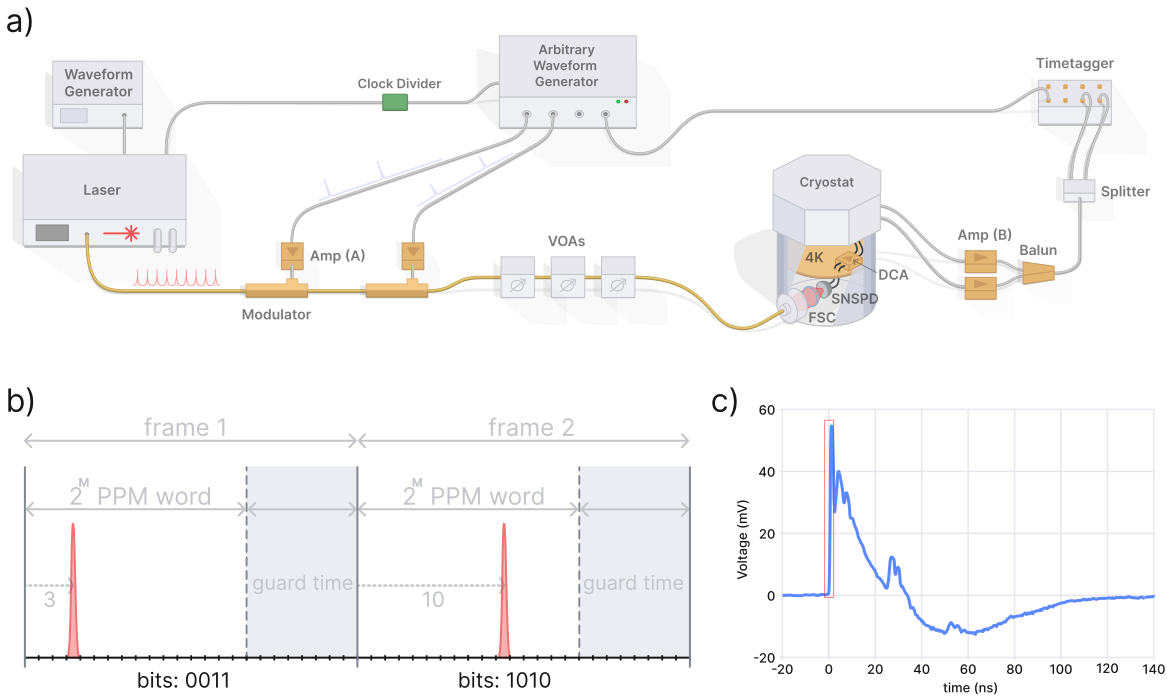
\includegraphics[width=1\textwidth]{./figs/fig_intro_2_light.pdf}
\caption[{PPM modulation and experiment setup}]{\textbf{PPM modulation and experiment setup} a) Diagram of the expiremental setup. WG: wave generator, CD: clock divider board, AWG: Arbitrary Waveform Generator, MLL: Mode Locked Laser (Pritel UAC), IM: Intensity Modulator, BC: Bias Controller, FSC: Free Space Coupling System, DCA: DC Coupled Cryo-amp b) How bits are transmitted in M=16 PPM modulation. An optical pulse is transmitted with a clock-referenced integer delay which encodes 4 bits of data. c) Scope trace of the RF pulse produced by the differential-readout tapered SNSPD. fig.~\ref{fig:waveform} zooms in on the rising edge outlined in red here}
\label{fig:intro}
\end{figure}
}

However, these detectors exhibit photon number number dependent responses that affect the time-correlated measurements needed for high-rate PPM. This behavior, shown in Fig.~\ref{fig:waveform} is also known as photon number resolution (PNR) -- a property that is desirable in certain applications including quantum communication and quantum computing. The SNSPD generates RF pulses with greater amplitude and slew rate when detecting optical pulses with multiple photons. Photon number effects are especially evident in this lower jitter variety of SNSPD due to the use of impedance matching tapers which more efficiently couple energy out of the nanowire and into the readout circuit. With high resolution time tagging equipment, photon number dependent effects have even been observed in SNSPDs not necessarily designed to exhibit it \cite{schapeler2023superconducting, sauer2023resolving} like those without tapers \cite{Cahall2017SlewRatePNR}. Therefore it is increasingly likely that future research involving low-jitter SNSPDs and multiphoton pulsed sources will have to explicitly manage the PNR response for accurate time-correlated measurements -- whether the effect it is desired or not.

For the tapered differential detectors, the PNR response affects timing of fixed threshold timetaggs at any trigger level (fig.~\ref{fig:waveform}). However, at higher trigger levels the PNR response is less pronounced and the timing measurements are less affected. Therefore, we divide a single SNSPD readout line using an RF splitter and trigger on the RF pulse at a high and low level as shwon by the red lines in fig.~\ref{fig:waveform}. This allows us to extract the somewhat conjugate information of pulse arrival time and photon number. From these measurements we study the PNR response in detail and present two methods for managing it. We demonstrate how the photon number information may be deconvolved from the arrival time information, and how both de-correlated degrees of freedom can be extracted simultaneously. This enables the original goal of high rate PPM, but also informs how low-jitter photon number resolving SNSPDs can be used in other classical communication and quantum applications.

\hypertarget{fig:waveform}{%
\begin{figure}
\centering
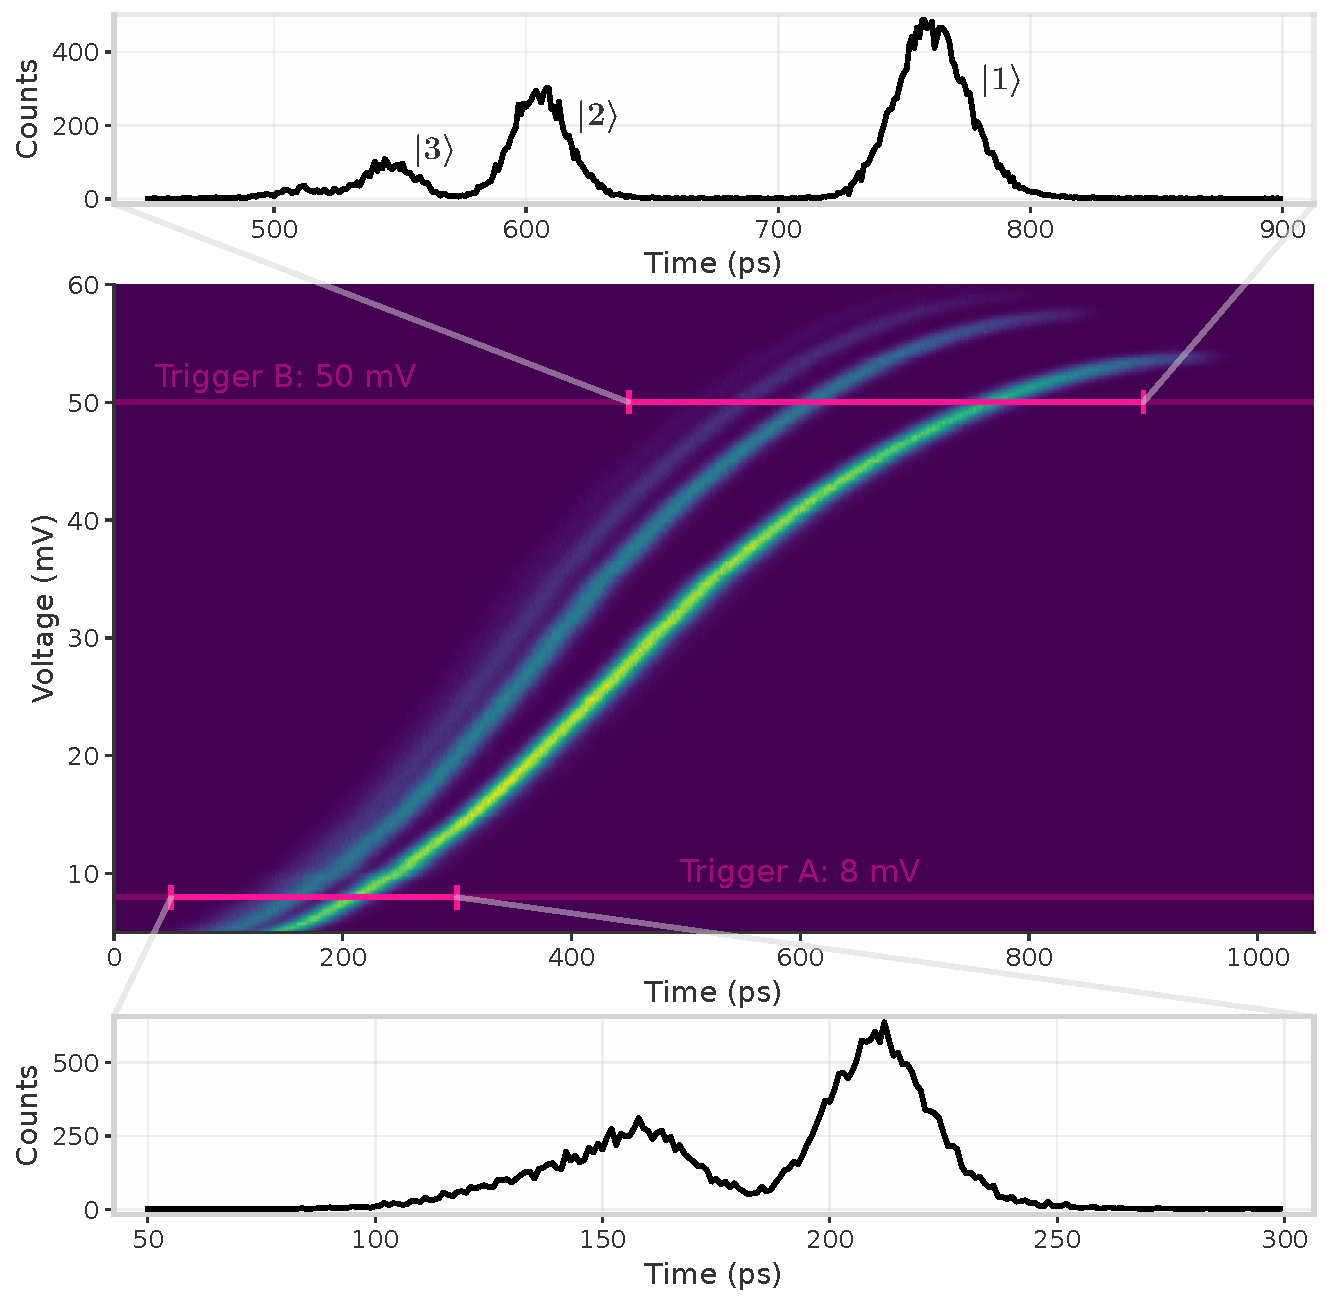
\includegraphics[width=0.8\textwidth]{./figs/waveform_light.pdf}
\caption[{PNR-sensitive Pulse Waveform}]{\textbf{PNR-sensitive Pulse Waveform} The rising edge of the differential SNSPD's RF pulses exhibit variations in height, slew rate, and arrival time due to photon-number dependent dynamics. The slopes of the 1-photon and 2-photon pulses significantly differ, and as the photon number increases, the alterations to the pulse shape become progressively smaller. Trigger levels A (8~mV) and B (50~mV) were used to extract as much information about pulse slope and arrival time as possible}
\label{fig:waveform}
\end{figure}
}

\hypertarget{detector-figure-of-merit}{%
\section{Detector Figure of Merit}\label{detector-figure-of-merit}}

The work here highlights the application of low jitter single-photon detectors for optical communication, which is impactful for deep-space optical communication as well as classical communication in quantum networks. Although single-photon counting is well estanblished for deep-space optical communication~\cite{Srinivasan2023GroundReceiver} so far it has not been ulitized in quantum networks, mainly due to the use of SFP modules and DWDMs. However, with the eachievement of high data rates recently achieved with photon-counting classical communication, these approaches can now be seriously considered for quantum networks. The main driver is the reduction of optical power in neighbouring DWDM channels, which ultimately lowers the Raman scattered photons into the quantum channel \cite{EraerdsRaman}
\textbf{\hl{Calculate reduction in power from state of the art SFP modules}}

To access the applicability of different detectors, here we compare some of the recent near infrared detectors.

A useful figure of merit that includes all of the revelant detector metrics for photon timing was introduced by Bronzi and co-authors \cite{Bronzi2016}

$$FoM_T = \frac{\eta  (1 - P_{ap})\Phi_{-3 \text{dB}}}{J} \sqrt{\frac{A}{D}},$$

where $\eta$ is the single photon detection efficiency, $\Phi_{-3 \text{dB}}$ is the photon flux at which the system detection efficiency drops by 3~dB, $P_{ap}$ is the afterpulsing probability, $J$ is the detector jitter evaluated as the FWHM, $T_d$ is the deadtime, $A$ is the active area and $D$ is the dark count rate. Here we have defined the maximum photon flux as the 3~dB point, for ease of standardization.

In this work:

\begin{itemize}
\tightlist
\item
  Efficiency = 0.84
\item
  Afterpulsing = 0 %
\item
  Jitter = 15 ps
\item
  Deadtime = 30 ns \textbf{\hl{measure 3dB flux}}
\item
  Area = 330 $\mu m^2$
\item
  Dark count rate = 20~Hz
\end{itemize}

$FoM_T = 7.58 \times 10^{12}$ at 1550 nm.

The deadtime is calculated as the 1/MCR, which is the 3 dB point of the nominal efficiency. This is only a factor of 3.7 less than the state of the art visible Silicon SPADs (peak efficiency at 480~nm) \cite{Gramuglia2022}

In the future, the performance of the optical communication system could be improved by using, high count rate SNSPD arrays. Recently published high-count rate arrays have figures of merit of \textbf{\hl{$FoM_T$ for Peacoq and Resta2023 results}}. This would result in a proportinal increase in the data rate.
\textbf{\hl{$FoM_T$ for fastest InGaAs/InP gated detector}}
These devices are ideal for fiber-based optical communication. In free-space, the active area is especially important, whithout the use of an adaptive optics system.
\textbf{\hl{$FoM_T$ for DSOC array}}

\hypertarget{development-of-a-modulation-source}{%
\subsection{Development of a modulation source}\label{development-of-a-modulation-source}}

DSOC relies on modulation of a CW seed laser to generate the communication signal on the spacecraft. This signal is then amplified by an Erbium Doped Fiber Amplifier (EDFA) to increase its transmission power to Earth. As the EDFA amplifies the pre-generated pulses and uses most of the power of the spacecraft optical transmission system, power consumption scales with the number of optical pulses.

We produce our PPM signal signal by carving a high rate mode locked laser with lithium niobate modulators. This way, the jitter of the optical pulses themselves are not limited by the modulators or slew slew rate of the RF signal that drives them. We do two PPM demonstrations, with the source mode locked laser operating at 10.75 and 20 GHz. THe 10.75 GHz demonstration uses a M value of 10, thereby making frames with 1024 time slots of 93 ps width each. The 20 GHz demonstration uses M=11, giving 2048 time slots of 50 ps width per frame. Each frame ends with a dead time of approximately 150 ns to allow the SNSPD to fully recover before the next frame.

Several modern free running time taggers support the averaging of multiple input channels to create fewer higher resolution channels. This implies a tradeoff between jitter or timing resolution and number of channels for a given time tagging device. Therefore, it is important to consider readout methods like that presented here that make use of 2 lower-resolution channels in place of a single higher resolution channel, as these two configurations are similarly resource efficient.

\hypertarget{methods}{%
\section{Methods}\label{methods}}

Prior to the PPM demosntration, we collected data with multi-photon optical pulses repeatedly impinging on the detector at the same time with respect to a clock. This way, we study how the PNR effect in isolation is manifest in the timing measurements recorded at the low and high trigger levels. We label the measurements from the low (8~mV) and high (50~mV) trigger levels as $t_A$ and $t_B$ respectively. As shown in Fig.~\ref{fig:waveform}, histograms of these arrival events are multimodal due to the PNR response. We first present a method for recovering a symmetric arrival time response function using the the slope measurement $\Delta t_{BA} = t_B - t_A$.

\hypertarget{slope-based-correction}{%
\subsection{Slope-Based Correction}\label{slope-based-correction}}

\hypertarget{fig:slope_correction}{%
\begin{figure}
\centering
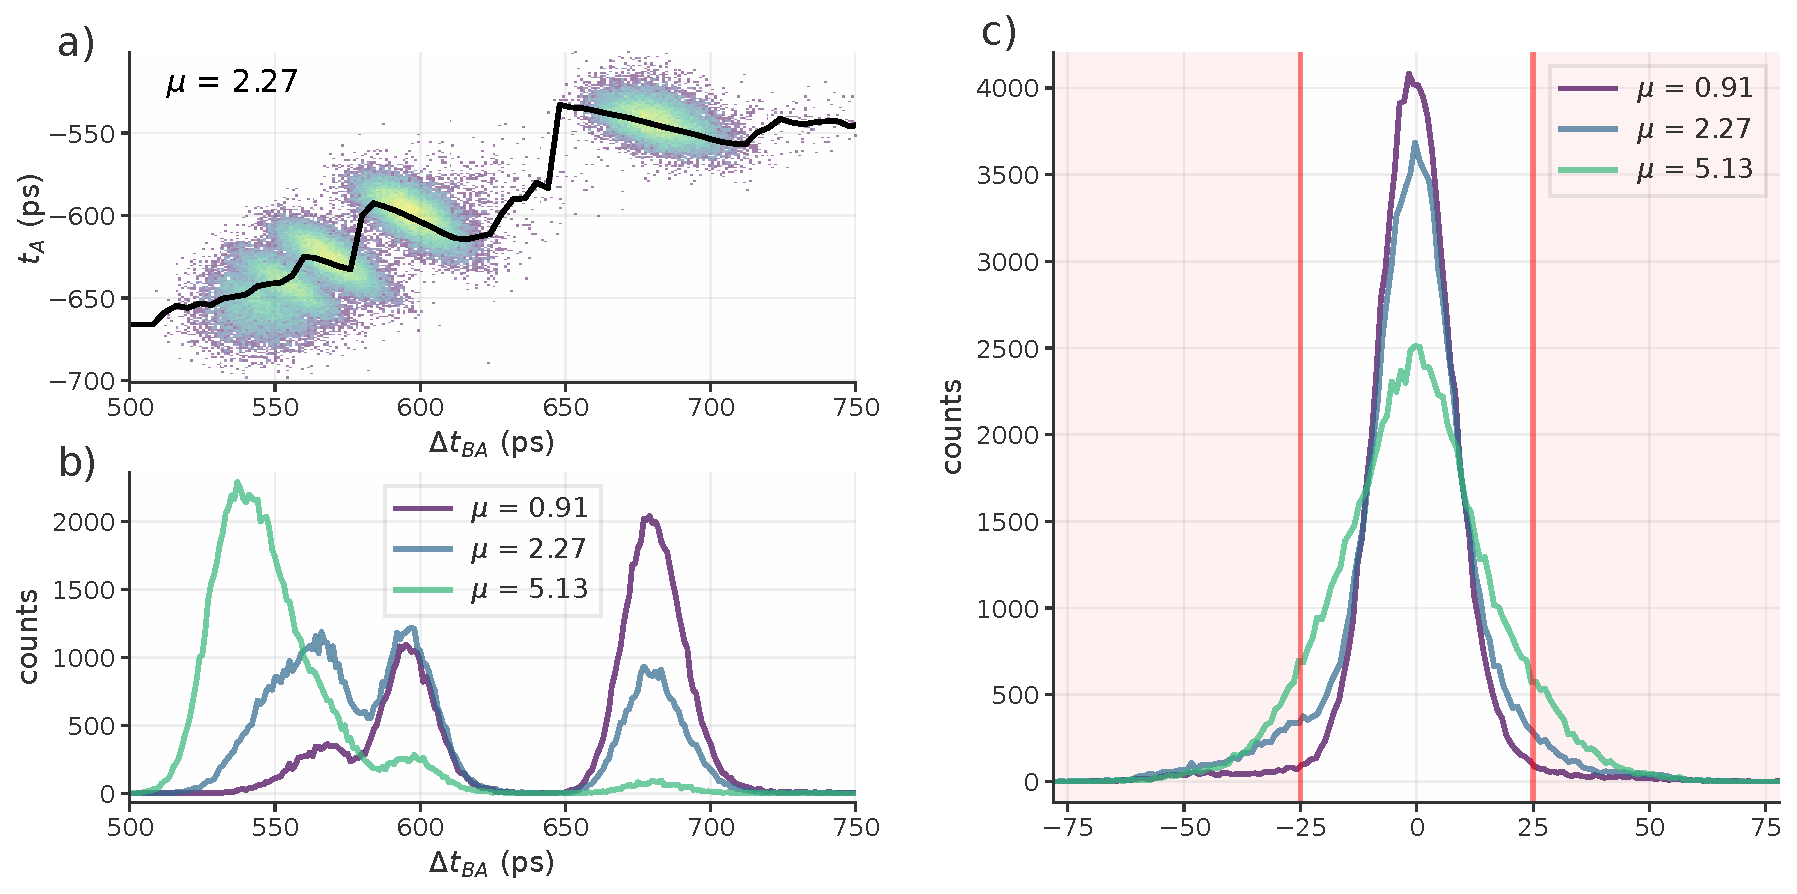
\includegraphics[width=1\textwidth]{./figs/slope_cancellation_light.pdf}
\caption[{PNR Slope Variation Analysis and Cancellation}]{\textbf{PNR Slope Variation Analysis and Cancellation} a) 2D histogram of RF pulse measurements. Through graphing slope $\Delta t_{BA}$ on the x-axis and arrival time $t_A$ on the y-axis, a series of groupings are visible that identify the discrete photon numbers detected.}
\label{fig:slope_correction}
\end{figure}
}

Pairs of pulse measurements $t_A$ and $t_B$ may be graphed on a 2D plane parametrized by $\Delta t_{BA}$ on the x-axis and $t_A$. fig.~\ref{fig:slope_correction} a shows how this protection exhibits multiple groupings that correspond the the photon number character of the impinging optical mode. The 1 and 2-photon events are clearly identifiable and seperated from other events, with $|3\rangle$, $|4\rangle$, and $|5\rangle$ events also visible with less mutual separation. While fig.~\ref{fig:slope_correction} a is shown here for just one mean photon number $\mu$, these grouplings are collected for a full range of attenuations and corresponding $\mu$. fig.~\ref{fig:slope_correction} a shows histograms from projecting 3 such groupings down onto the $\Delta t_{BA}$ axis.

Thee slope correction method involves the measurement and creation of a slope-versus-arrival time line, one of which is shown in fig.~\ref{fig:slope_correction} a. This is produced by averaging all $t_A$ measurements for a given slope $\Delta t_{BA}$. That is, the values along vertical slices of the 2D density plot in fig.~\ref{fig:slope_correction} a are averaged to produce the y-coordinates of the slope-versus-arrival time line shown in black. By interpolating new $\Delta t_{BA}$ measurements on this curve and using it like a lookup table, PNR corrections $C_A$ are found. These may be subtracted off from $t_A$ producting $\tilde{t_A} = t_A - C_A(\Delta t_{BA})$ where $\tilde{t_A}$ is a constructed timing measurement that exhibits a symmetric arrival time response function and shown in fig.~\ref{fig:slope_correction} c.~

The data representation and calibration curve shown in fig.~\ref{fig:slope_correction} a may be constructed with $t_B$ on the y-axis as well. Then the PNR corrections are applied the the $t_B$ measurements instead. However, the resulting histograms $\tilde{t_B}$ are virtual identical to $\tilde{t_A}$.

\hypertarget{cluster-analysis}{%
\subsection{Cluster Analysis}\label{cluster-analysis}}

\hypertarget{results}{%
\section{Results}\label{results}}

results here

{}


\bibliography{references}



\end{document}